\documentclass[UTF8]{ctexart}
\usepackage{booktabs}
\usepackage{cleveref}
\usepackage{graphicx}
\title{这里是标题}
\author{这里是作者}
\date{2019.9.21}
\begin{document}
\maketitle
\begin{abstract} 
这里是摘要

\textbf{关键词:}关键词一\quad 关键词二
\end{abstract}
\section{这里是关键词一\quad 关键词二要一段}
\subsection{第一段的第一子段}
\subsubsection{第一小节}
你好世界\cite{Liu},
单个回车
不会换行
\subsubsection{第二小节}
需要两个回车


才能换行
\subsection{第一段的第二子段}
\section{第二段}
表格引用测试\cref{tbl:number};
图片引用测试\cref{fig:function}
这里是行间公式$A_{ij}^n \quad \delta \pi \partial \sigma   \epsilon \alpha  \beta \gamma \Delta \Pi \times \div$
\begin{equation}
\alpha^2 + \beta^2 = \gamma^2
\end{equation}
\[ \int_0^1f(x)dx=lim_{x \to \infty}\sum_{i-1}^nf(\frac{i}{n}) \]
\[ \int_0^1f(x)dx=\lim\limits_{x \to \infty}\sum\limits_{i-1}^nf(\frac{i}{n}) \]   

\begin{table}
\caption{这里是表格}
\label{tbl:number}
\begin{center}
\begin{tabular}{lcr}
\toprule
One & Two & Three \\
\midrule
A & 1 & Alpha \\
B & 2 & Beta \\
C & 3 & Sigma \\
\bottomrule
\end{tabular}
\end{center}
\end{table}

\begin{figure}
    \centering
    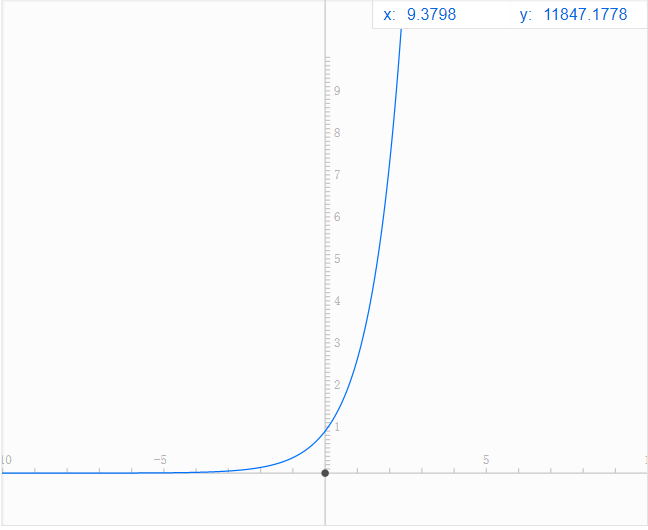
\includegraphics[width=.7\textwidth]{imgs/ex.png}
    \caption{$y=e^x$图像}
    \label{fig:function}
\end{figure}

\begin{thebibliography}{9}
    \bibitem[1]{Liu} 刘海洋. \LaTeX 入门[M]. 北京: 电子工业出版社, 2013.
    \bibitem[2]{Hu} 胡伟. \LaTeX 2e完全学习手册(第二版). 北京: 清华大学出版社, 2013.
\end{thebibliography}
\end{document}